\paragraph{QuizziPedia::Back-End::App::Routers::LangRouter}
\label{QuizziPedia::Back-End::App::Routers::LangRouter}
\begin{figure}
	\centering
	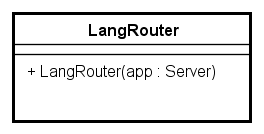
\includegraphics[scale=0.45]{UML/Classi/Back-End/QuizziPedia_Back-End_App_Routers_LangRouter.png}
	\caption{QuizziPedia::Back-End::App::Routers::LangRouter}
\end{figure}
\FloatBarrier
	\begin{itemize}
		\item \textbf{Descrizione} \\
		Classe che gestisce le richieste relative alla lingua.
		\item \textbf{Utilizzo} \\
		Viene utilizzata per chiamare il controller che si occupa di cambiare la lingua dell'applicazione.
		\item \textbf{Relazioni con altre classi}
			\begin{itemize}
				\item \textbf{IN \texttt{Server}} \\
				Classe che avvia il server. Nello specifico apre una connessione al database tramite \textit{Mongoose\ped{G}}, invoca il middleware\ped{G} \textit{Express\ped{G}} passando un riferimento al database MongoDB come parametro in modo che possa configurarsi con esso, invoca il middleware\ped{G} \textit{Passport\ped{G}} ed infine si mette in ascolto su una determinata porta. è il componente \textit{client\ped{G}} del pattern \textit{Chain of responsability\ped{G}}. Utilizza i moduli \textit{Mongoose\ped{G}}, \textit{Express\ped{G}}, \textit{Passport\ped{G}}.
				\item \textbf{OUT \texttt{NotFoundHandler}} \\
				Classe che si occupa della gestione dell'errore di una pagina non trovata. Componente ConcreteHandler del design pattern Chain of responsability.
			\end{itemize}
		\item \textbf{Metodi}
			\begin{itemize}
				\item \texttt{+ LangRouter(app: Server)} \\
				Contiene diverse ruote che vengono configurate all'avvio del server. Quest'ultime ricevono le richieste del \textit{client\ped{G}} e passano il controllo al ConcreteHandler successivo. \\
				\textbf{Parametri}:
					\begin{itemize}
						\item \texttt{app: Server} \\
						Rappresenta l'istanza del server su cui configurare i ruote che mappano i controllers specifici.
					\end{itemize}
			\end{itemize}
	\end{itemize}